\section{Experimentos e resultados}
\subsection{Experimentos}
A fim de poder entender o funcionamento do simulador NS-2 e tamb\'em estudar simula\c{c}\~oes de comunica\c{c}\~ao em cen\'arios militares, foram definidos 2 experimentos te\'oricos, sendo o Experimento 1, um teste simples de converg\^encia de rotas, e o Experimento 2, baseado em estudos realizados por \cite{pereira}, o qual representa um caso de assalto e tomada de posi\c{c}\~ao inimiga.

Cada experimento possui suas caracter\'isticas, mas exitem uma semalhan\c{c}a base, que \'e o tr\'afego que ir\'a caminhar pela rede, como comentado na se\c{c}\~ao \ref{trafegoDados}, o qual foi escolhido o CBR.

\subsubsection{Experimento 1}
O experimento 1 baseia-se na ideia simples de um protocolo de rede \textit{ad hoc}, roteamento din\^amico.
O objetivo principal deste experimento \'e poder analizar o tempo de converg\^encia de roteamento de uma origem a um destino, alterando uma vez o caminho pelo qual eles realizam a comunica\c{c}\~ao.
A Tabela \ref{tabParamExp1} demonstra resumidamente os par\^ametros utilizados na execu\c{c}\~ao do experimento 1.

\begin{table}[H]
	\centering
	\caption{Resumo dos par\^ametros usados no Experimento 1.}
	\begin{tabular}{ | l | l | }
		\hline
		N\'umero total de n\'os & 4 \\ \hline
		N\'umero de fontes de tr\'afego & 1 \\ \hline
		N\'umero de conex\~oes & 1 \\ \hline
		Tempo de simula\c{c}\~ao & 300 segundos \\ \hline
		\'Area total da simula\c{c}\~ao & 500x500 metros \\ \hline
		Tamanho dos pacotes & 512 \textit{bytes} \\ \hline	
		Velocidade dos n\'os & 1.5m/s constante \\ \hline
		Velocidade de banda & 11Mbps/s \\ \hline
	\end{tabular}
	\label{tabParamExp1}
\end{table}

A Figura \ref{figExp1} demonstra o experimento realizado, onde cada Soldado(n\'o) deve atingir seu respectivo Destino.
Cada Soldado inicia seu movimento a um tempo determinado na simula\c{c}\~ao, onde na Figura \ref{figExp1} \'e referenciado pelo prefixo \textit{at}, o qual \'e defido em segundos, e abaixo exibe o movimento de cada Soldado, onde nesse experimento todos os Soldados possuem um movimento constante de 1,5 metros por segundo. 

A fonte de tr\'afego nesse experimento \'e somente de uma, a qual realiza uma conex\~ao do Soldado 3(fonte) ao Soldado 1(destino). Inicialmente vai passar pelo Soldado 2 essa comunica\c{c}\~ao, pois os Soldados 1 e 3 n\~ao est\~ao pr\'oximos a fim de criarem uma rota direta.

\begin{figure}[H]
	\centering
	\includegraphics[scale=0.5]{experimento1.eps}
	\caption{Experimento 1}
	\label{figExp1}
\end{figure}

Observe que o Soldado 4 inicia somente seu movimento ao tempo de 150,0 segundos, enquanto os demais Soldados iniciam seus movimentos ao instante de 0,1 segundos.
Isso foi definido pelo fato do tempo em que o Soldado 2 atinja seu objetivo e pare de seguir em frente, enquanto os Soldados 1 e 3 continuam seus movimentos, e possam alcan\c{c}ar e estar dentro do raio de comunica\c{c}\~ao com o Soldado 4.
Quando os Soldados 1 e 3 se afastam do Soldado 2, eles perdem a sua rota por esse \textit{host} da rede, e necessitam buscar uma nova rota, a qual seguir\'a pelo Soldado 4, e \'e nesse ponto onde cada protocolo dever\'a gerar resultados distintos.

\subsubsection{Experimento 2}
O experimento 2 foi baseado em estudos realizados por \cite{pereira} em sua tese de mestrado. 
O objetivo deste experimento \'e analizar o desempenho dos protocolos de roteamento como um todo em um cen\'ario militar. 
\cite{pereira} comenta que esse \'e um cen\'ario t\'ipico de simula\c{c}\~ao de uma opera\c{c}\~ao de assalto e tomada de posi\c{c}\~ao inimiga.

Esse cen\'ario consiste em 4 grupos de soldados e 1 ve\'iculo de apoio, e cada grupo de soldados \'e formado por 4 soldados.
Cada grupo possui um comandante, o qual envia ordens aos outros soldados do grupo, e tamb\'em recebe e envia ordens do ve\'iculo de apoio, este qual \'e encarregado de repassar as ordens aos demais grupos.
Cada grupo nesse cen\'ario tem como objetivo tomar a posi\c{c}\~ao inimiga, onde na Figura \ref{figExp2} est\'a descrito como "Destino final".

\begin{figure}[H]
	\centering
	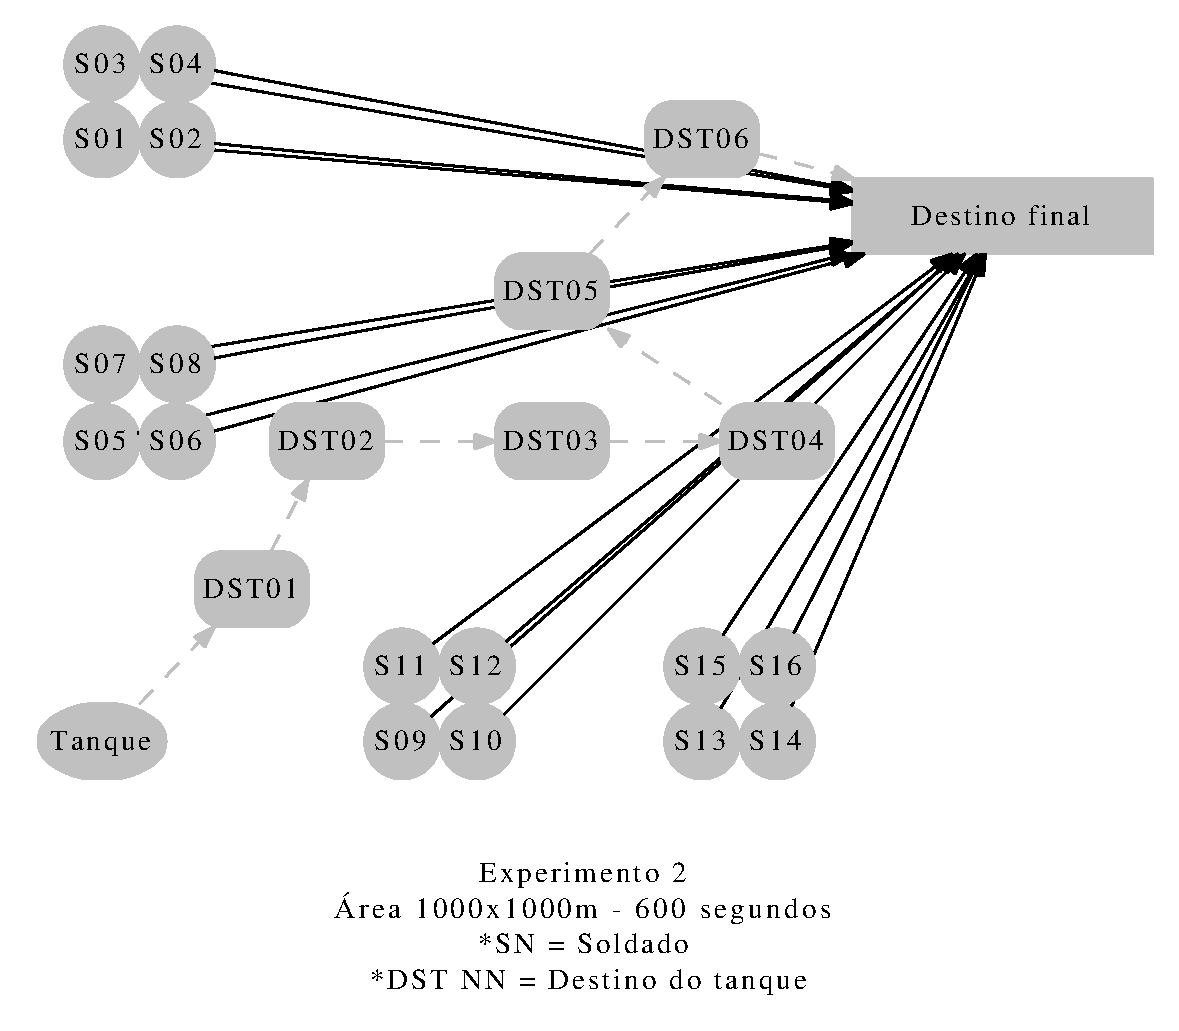
\includegraphics[scale=0.5]{experimento2.eps}
	\caption{Experimento 2}
	\label{figExp2}
\end{figure}

Todos os soldados de cada grupo dever\~ao avan\c{c}ar juntos durante o percurso do cen\'ario, n\~ao executando necess\'ariamente um caminho reto durante todo o trajeto.

A Tabela \ref{tabParamExp2} demonstra resumidamente os par\^ametros utilizados nesse experimento. 
Al\'em do tamanho e n\'umero de conex\~oes e n\'os diferentes do experimento 1, podemos verificar que a velocidade dos n\'os possue uma varia\c{c}\~ao.
Essa varia\c{c}\~ao ocorre pelo fato de que, os soldados recebem ordens de parada ou avan\c{c}o no percurso, sendo que em cada situa\c{c}\~ao \'e necess\'ario almentar, dimunuir ou at\'e mesmo parar o ritmo de avan\c{c}o no objetivo do cen\'ario.

\begin{table}[H]
	\centering
	\caption{Resumo dos par\^ametros usados no Experimento 2.}
	\begin{tabular}{ | l | l | }
		\hline
		N\'umero total de n\'os & 17 \\ \hline
		N\'umero de fontes de tr\'afego & 7 \\ \hline
		N\'umero de conex\~oes & 16 \\ \hline
		Tempo de simula\c{c}\~ao & 600 segundos \\ \hline
		\'Area total da simula\c{c}\~ao & 1000x1000 metros \\ \hline
		Tamanho dos pacotes & 512 \textit{bytes} \\ \hline
		Velocidade dos n\'os & 0 \`a 8 m/s constante \\ \hline
		Velocidade de banda & 11Mbps/s \\ \hline
	\end{tabular}
	\label{tabParamExp2}
\end{table}


\subsection{M\'etricas de desempenho}
Com base nos estudo de \cite{pereira} e \cite{schimidt} e informa\c{c}\~oes obtidas por \cite{salles} descritos na se\c{c}\~ao \ref{requisitos}, foram definidas m\'etricas para analizar o comportamento de cada protocolo.

\begin{itemize}
	\item \textbf{Taxa de entrega de pacotes:} Raz\~ao entre o n\'umero de pacotes entregues para o destino final e o n\'umero de pacotes gerados pela aplica\c{c}\~ao na fonte.
	\item \textbf{Atraso m\'edio fim a fim dos pacotes de dados:} Inclui todos os poss\'iveis atrasos causados pela lat\^encia da descoberta de rotas, propaga\c{c}\~ao, atrasos devido a retransmiss\~oes da camada MAC e tempos de transfer\^encia.
	\item \textbf{N\'umero de pacotes de roteamento:} \'E medido a quantidade total de pacotes de roteamento, representada pelos pacotes de descoberta e manuten\c{c}\~ao das rotas enviados pela origem ou encaminhados pelos n\'os intermedi\'arios. No protocolo por demanda (AODV), esses pacotes s\~ao representados pelos pacotes RREQ, RREP e RERR. No DSDV e OLSR, esses pacotes s\~ao representados pelas tabelas de roteamento que s\~ao trocadas periodicamente.
	\item \textbf{N\'umero de \textit{bytes} de roteamento:} \'E medido a quantidade total de \textit{bytes} em cada pacote de, incluindo a quantidade de \textit{bytes} de cabe\c{c}alho em pacotes de dados, que corresponde, normalmente, ao roteamento na fonte.
\end{itemize}
Segundo \cite{pereira}, o tr\'afego referente ao roteamento deve ser o menor poss\'ivel quando comparado ao tr\'afego de dados, pois para se enviar pacotes de roteamento gasta-se energia dos n\'os e consome-se banda, que s\~ao recursos escassos em redes sem fio. 
Para as redes militares, a taxa de entrega e o atraso s\~ao as m\'etricas mais importantes.

\subsection{An\'alise comparativa dos resultados}
As Figuras \ref{fig:resulExp1} e \ref{fig:resulExp2} apresentam atrav\'es de gr\'aficos os resultados obtidos dos experimentos executados. Esses resultados possibilitaram a formula\c{c}\~ao das conclus\~oes apresentadas mais adiante nesse trabalho.

\subsubsection{Experimento 1}
Nos gr\'aficos da figura \ref{fig:resulExp1} \'e poss\'ivel notar que n\~ao houveram muitas diferen\c{c}as entre os dados dos diferentes protocolos. A ideia do experimento aqui apresentado \'e testar o tempo de converg\^encia, o qual nos gr\'ficos \'e representado pela Figura \ref{fig:resulExp1}(b).

\begin{figure}[H]
	\centering
	\subfigure[Taxa de entrega de pacotes]{
		\includegraphics[scale=0.55]{exp1_taxa.eps}
	}\label{subfig:exp1Lost}
	\subfigure[Atraso m\'edio (ms)]{
		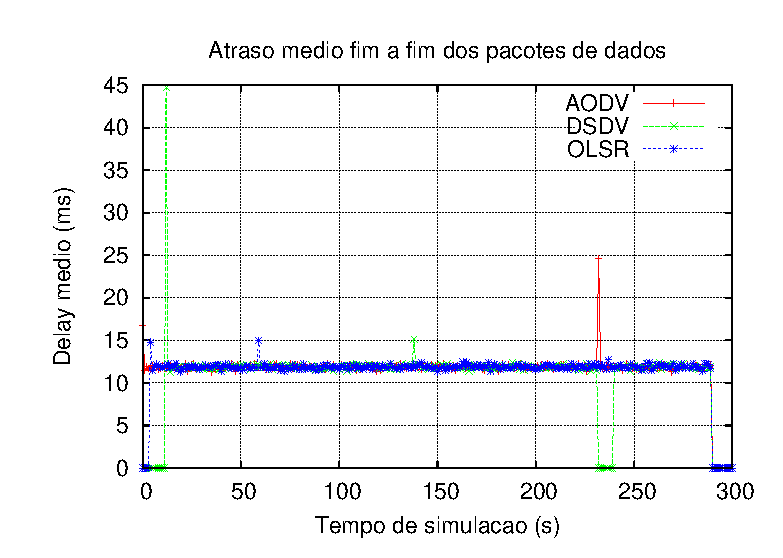
\includegraphics[scale=0.55]{exp1_delay.eps}
	}\label{subfig:exp1Late}
	\subfigure[N\'umero de \textit{bytes} de roteamento]{
		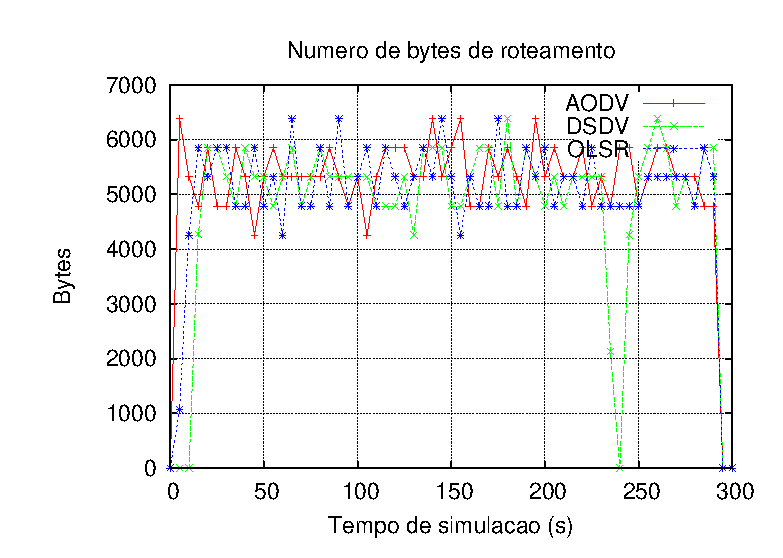
\includegraphics[scale=0.55]{exp1_byte.eps}
	}\label{subfig:exp1Byte}
	\subfigure[N\'umero de pacotes de roteamento]{
		\includegraphics[scale=0.55]{exp1_pkts.eps}
	}\label{subfig:exp1Pkts}
	
	\caption{Resultados para o experimento 1}
	\label{fig:resulExp1}
\end{figure}

Podemos perceber que a cada instante de tempo, temos pequenas diferen\c{c}as de roteamento, estes representados pelos gr\'aficos (c) e (d) da Figura \ref{fig:resulExp1}. A Tabela \ref{tabExp1Result} demonstra melhor estes resultados, sendo o resultado do total de dados trafegados pela rede no experimento 1.

\begin{table}[H]
	\centering
	\caption{Resultado das simula\c{c}\~oes do experimento 1}
	\begin{tabular}{ | l | l | l | l | }
		\hline
		M\'ETRICAS AVALIADAS & DSDV & AODV & OLSR \\ \hline
		Taxa de entrega & 92.98\% & 99.83\% & 98.43\% \\ \hline
		Atraso m\'edio (ms) & 10.7575 & 11.4837 & 11.3047 \\ \hline
		N\'umero de pacotes & 543 & 588 & 565 \\ \hline
		N\'umero de \textit{bytes} & 288896 & 312816 & 300580 \\ \hline
	\end{tabular}
	\label{tabExp1Result}
\end{table}

Podemos analizar que o DSDV obt\'em uma r\'apida vantagem em n\'umero de pacotes e \textit{bytes} gerados no experimento em rela\c{c}\~ao aos demais protocolos. Por\'em essa r\'apida vantagem \'e anulada pela taxa de entrega, que foi bem menor em rela\c{c}\~ao ao protocolo AODV e OLSR.

O objetivo inicial desse experimento era analizar o tempo de converg\^encia entre os protocolos, o qual n\~ao foi muito significativo, pois resultou em diferen\c{c}as menores de 1 ms entre os protocolos de roteamento. 
O destaque nesse experimento ficou na taxa de entrega, pois demonstra que o OLSR e p AODV mantiveram uma taxa pr\'oximo de 100\%, e o DSDV obteve uma taxa inferior.

\subsubsection{Experimento 2}
Diferentemente do experimento 1, o experimento 2 possui caracter\'isticas diferentes de mobilidade, onde cada soldado no cen\'ario n\~ao vai percorrer um caminho cont\'inuo e tamb\'em n\~ao vai ter uma velocidade constante de avan\c{c}o para o objetivo final do cen\'ario.
A fim de trazer uma m\'edia de resultados satisfat\'orios, foram gerados e executados simula\c{c}\~oes de cen\'arios 15 vezes, a fim de obter uma m\'edia somat\'oria entre os dados.
Os gr\'aficos da Figura \ref{fig:resulExp2} demonstram os resultados obtidos no experimento 2.

\begin{figure}[H]
	\centering
	\subfigure[Taxa de entrega de pacotes]{
		\includegraphics[scale=0.55]{exp2_taxa.eps}
	}\label{subfig:exp2Taxa}
	\subfigure[Atraso m\'edio (ms)]{
		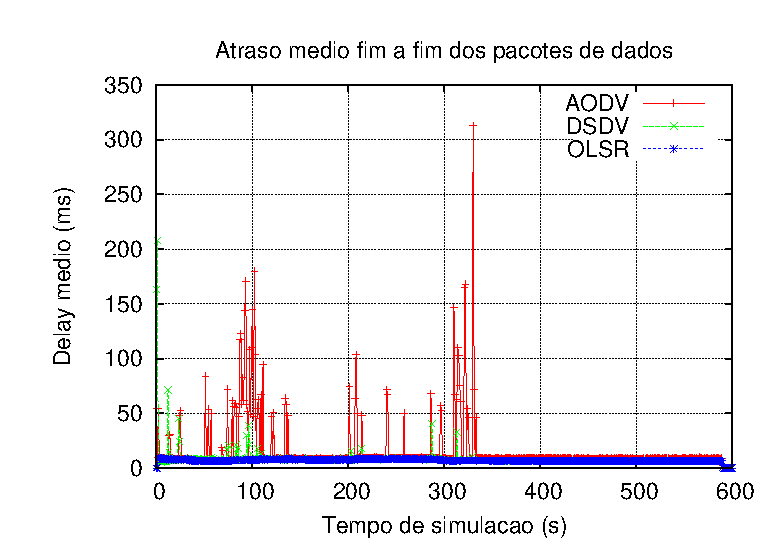
\includegraphics[scale=0.55]{exp2_delay.eps}
	}\label{subfig:exp2Late}
	\subfigure[N\'umero de \textit{bytes} de roteamento]{
		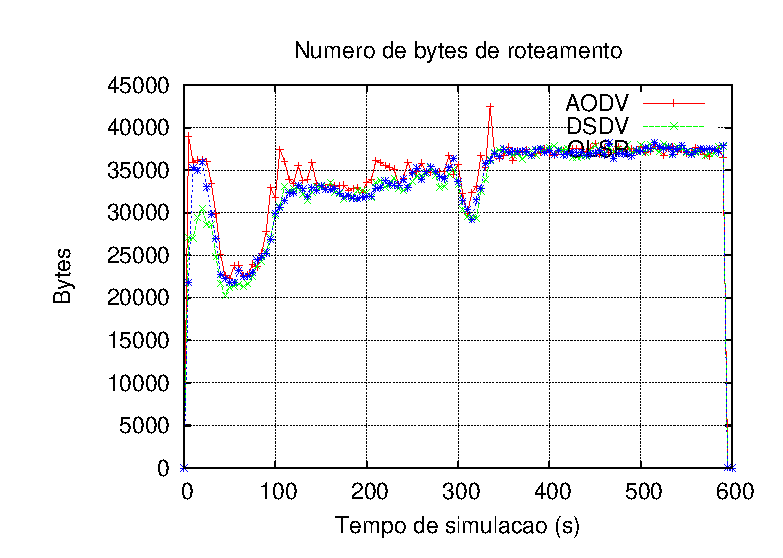
\includegraphics[scale=0.55]{exp2_byte.eps}
	}\label{subfig:exp2Byte}
	\subfigure[N\'umero de pacotes de roteamento]{
		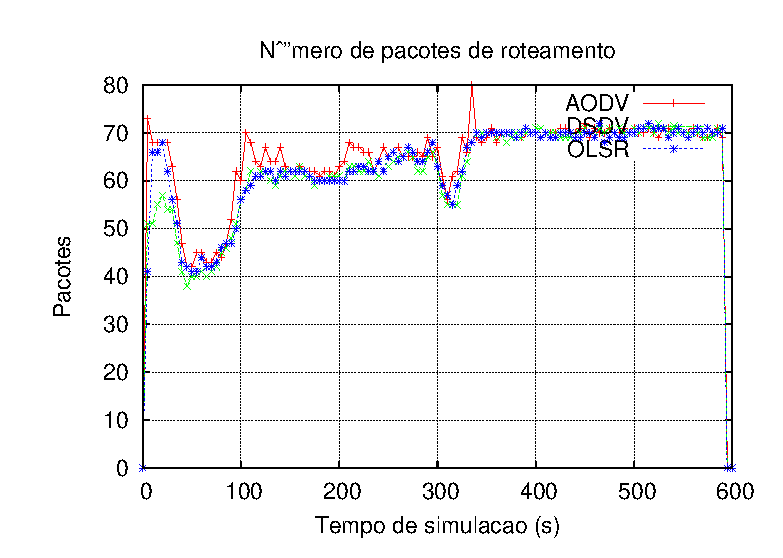
\includegraphics[scale=0.55]{exp2_pkts.eps}
	}\label{subfig:exp2Pkts}
	
	\caption{Resultados para o experimento 2}
	\label{fig:resulExp2}
\end{figure}

Com rela\c{c}\~ao as Figuras \ref{fig:resulExp2}(c) e \ref{fig:resulExp2}(d), o comportamento \'e similar, pois como cada pacote tem um tamanho fixo de 512 \textit{bytes}, o n\'umero de \textit{bytes} de roteamento vai ser proporcional ao n\'umero de pacotes de roteamento.

Em rela\c{c}\~ao a m\'etrica de Taxa de Entrega, podemos notar que h\'a pequenas oscila\c{c}\~oes, e que somente o protocolos AODV teve uma grande perda de informa\c{c}\~oes.

\begin{table}[H]
	\centering
	\caption{Resultado das simula\c{c}\~oes do experimento 2}
	\begin{tabular}{ | l | l | l | l | }
		\hline
		M\'ETRICAS AVALIADAS & DSDV & AODV & OLSR \\ \hline
		Taxa de entrega & 96.88\% & 90.37\% & 95.29\%  \\ \hline
		Atraso m\'edio(ms) & 8.15969 & 16.3527 & 6.88545  \\ \hline
		N\'umero de pacotes & 7407 & 7696 & 7483  \\ \hline
		N\'umero de \textit{MegaBytes} & 3.76 & 3.90 & 3.80  \\ \hline
	\end{tabular}
	\label{tabExp2Result}
\end{table}

A Tabela \ref{tabExp2Result} demonstra um resultado total do experimento 2. Nela podemos avaliar que o AODV teve um desempenho inferior no desempenho de entrega dos pacotes, que pode ser conferido na Figura \ref{fig:resulExp2}(b), gerou mais pacotes e teve uma taxa de entrega inferior.
